\documentclass[twoside,UTF8]{EPURapport}
\usepackage{listings}

%\renewcommand{\lstlistlistingname}{Liste des codes}
%\renewcommand{\lstlistingname}{Code}

%\addextratables{%
%	\lstlistoflistings
%}

%\swapAuthorsAndSupervisors




\thedocument{Rapport de Projet}{Batching et optimisation des trajectoires de picking dans un centre d'entreposage}{Batching et picking}

\grade{Département Informatique\\ 3\ieme{} année\\ 2008 - 2009}

\authors{%
	\category{Étudiants}{%
		\name{Shimeng ZHANG} \mail{shimeng.zhang@etu.univ-tours.fr}
		\name{Natacha MARLIO-MARETTE} \mail{natacha.marlio-marette@etu.univ-tours.fr}
	}
	\details{DI3 2012 - 2013}
}

\supervisors{%
	\category{Encadrants}{%
		\name{Ameur SOUKHAL} \mail{ameur.soukhal@univ-tours.fr}
	}
	\details{Université François-Rabelais, Tours}
}

\abstracts{Description en français}
{Mots clés français}
{Description en anglais}
{Mots clés en anglais}






\begin{document}

%%%%%%%%%%%%%%%%%%%% INTRODUCTION %%%%%%%%%%%%%%%%%%%%

\chapter{Introduction}

%%%%%%%%%%%%%%%%%%%% CHAPITRE 1 %%%%%%%%%%%%%%%%%%%%%%

\chapter{Présentation du projet}

\section{Définitions et mise en place du problème}
\subsection{Définitions}
\paragraph{}Dans cette partie, nous définirons quelques notions permettant une meilleure compréhension de ce rapport.
\begin{description}
\item[• Picking]: C'est l'opération qui consiste à prélever les articles dans la quantité demandé par la commande avant son expédition.

\item[• Cluster]: Ce terme peut être employé dans plusieurs domaines tels que les sciences, l'informatique ou bien la musique. Ici, un cluster correspond au regroupement des objets au ceint d'un ensemble.
\item[• Heuristique] : Une heuristique est une méthode de calcul qui fournit rapidement une solution réalisable. Mais cette solution n'est pas nécessairement optimale. Ce terme s'applique pour un problème d'optimisation NP-difficile.
\end{description}


\subsection{Mise en place du problème }
\paragraph{}La problématique de ce projet est de trouver l'itinéraire que doit réaliser chaque chariot au ceint d'un entrepôt. Pour ce faire nous avons réaliser un programme en C qui définit la tournée que doit effectuer le chariot. Cependant nous avions quelques contraintes à respecter (cf la section \ref{sec:Contraintes} page \pageref{sec:Contraintes}). Pour cela nous avons utiliser différents heuristiques, il faudra par la suite en effectuant des tests déterminer le meilleur.


\section{Cahier des Charges}
\subsection{Cahier des Charges}
\paragraph{}Pour répondre à la problématique de ce projet, nous devions respecter un cahier des charges. Afin de trouver, l'itinéraire qu'emprunteront les chariots, nous avons utiliser différentes méthodes(cf les sections \ref{sec:CFRS} page \pageref{sec:CFRS} et \ref{sec:RFCS} page \pageref{sec:RFCS}). Nous avons considéré pour tout ce projet qu'un unique chariot et des objets avec un poids unique. 

\paragraph{}Pour chercher l'itinéraire de notre chariot, il faut tout d'abord lui dire ce qu'il doit aller chercher dans l'entrepôt. C'est à dire lui donner un carnet de commandes. Il faut connaître la position de chaque objet dans l'entrepôt ainsi que leur poids. Ces deux éléments seront donnés avec le carnet de commandes.

\paragraph{}Après la réalisation des différents heuristiques, il faudra faire une série de test de façon à savoir lequel est le meilleur des deux. Ces tests sont expliqués dans le chapitre \ref{chap:test} page \pageref{chap:test}.

\subsection{Contraintes}
\label{sec:Contraintes}
\paragraph{}Dans ce projet, il faut tenir compte de certaines contraintes : 
\begin{itemize}
\item[•]\textbf{La capacité du chariot}: En effet, celui-ci ne peut contenir qu'une certaine quantité (un certain poids).
\item[•]\textbf{La compatibilité et incompatibilité des produits} : Il faut tenir compte de la compatibilité des produits, de façon à ce qu'aucun produits ne soient écrasé dans le chariot.
\item[•]\textbf{Zone d'exclusion mutuelle}: Il faut synchroniser les itinéraires de façon à éviter que les chariots puissent entrer en collision. 
\item[•]\textbf{La cartographie de l'entrepôt} : Celle-ci étant inconnue, il est difficile de calculer un itinéraire exact pour le chariot. Ce qui a un impact sur la distance totale que le chariot devra parcourir.
\end{itemize} 

Nous n'avons pour ce projet tenu compte uniquement de la première contrainte.

\section{Différentes méthodes de batching et picking}

Il existe différentes méthodes de batching et picking. Durant ce projet, nous avons mis en œuvre les deux premières présentées ci-dessous.

\subsection{Cluster First Root Second}
\label{sec:CFRS}

\paragraph{}La méthode \textit{Cluster First Root Second} signifie que l'on s'occupe en premier des clusters et en second de l'itinéraire. C'est à dire que l'on découpe tout d'abord la commande en cluster. On va couper la commande à chaque fois que le chariot sera plein. Et ensuite l'on définit l'itinéraire de chaque cluster. 

\subsection{Root First Cluster Second}
\label{sec:RFCS}
\paragraph{}Cette seconde méthode \textit{Root First Cluster Second} est l'opposée de \textit{Cluster First Root Second}. En effet lors de son application, on ne va non plus déterminer en premier les différents clusters mais l'itinéraire de toute la commande. Puis par la suite, on va la découper à chaque fois que le chariot sera plein. Celui-ci pourra donc lors de ces coupures retourner au dépôt afin d'être vidé.




%%%%%%%%%%%%%%%%%%%% CHAPITRE 2 %%%%%%%%%%%%%%%%%%%%%%

\chapter{Cluster First Root Second}

\paragraph{} Ce chapitre présente le programme utilisant la méthode \textit{Cluster First Root Second}. 

\section{Architecture du programme}

\subsection{Structures de données}
\label{subsec:struct}

\paragraph{} Cette section a pour objectif de présenter les différentes structures de données utilisées pour la méthode \textit{Cluster First Root Second}.

\paragraph{}Ces différentes structures sont définies dans les fichiers suivant : 
\begin{itemize}
\item[•] \textit{util.h}
\item[•]\textit{ListeCluster.h}
\item[•]\textit{Cluster.h}
\item[•]\textit{Objet.h}
\end{itemize}
\subsubsection{Utile}

\paragraph{}
Un fichier \textit{util.h} a été crée pour gérer le type bool qui correspond au booléen. 
Ci-dessous la définition du type booléen. 
\begin{lstlisting}[caption ={Définition du type Booleen} , label ={listing : useless}]
typedef int bool;
#define TRUE 1
#define FALSE 0
\end{lstlisting}

Lorsque l'on attribue la valeur "TRUE" à une variable, celle-ci prend comme valeur "1". De m\^eme pour "FALSE", la variable prendra la valeur "0".


\subsubsection{ListeCluster}

\paragraph{}
ListeCluster est une liste cha\^inée qui a pour représentation :

\begin{figure}[!h]
\texttt{ListeCluster = \^\,Place;}
\paragraph{}
 \texttt{ Place = enregistrement 
\begin{description}
\item cap : Entier non signé;
\item succ : ListeCluster;
\item fini : Bool;
\item ptrC : Cluster;
\item fin; 
\end{description}
}
\caption{Représentation de la structure ListeCluster}
\end{figure}

\paragraph{}ListeCluster est une liste chainée de pointeurs vers une liste de type de structure Cluster. Cette structure sert à gérer les différents cluster. Chaque élément de la liste indique la capacité de son cluster avec l'attribut \"cap\". Mais aussi si le cluster peut contenir un autre produit avec l'attribut "fini". Celui-ci vaut "TRUE" lorque la capacité du cluster est égale à la capacité maximum du chariot.
Ci-dessous le graphe de collaboration de la structure.

\begin{figure}[!h]
\center
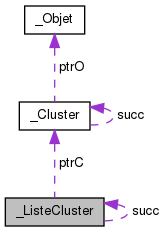
\includegraphics[scale=0.5]{images/struct_liste_cluster.png}
\caption{Graphe de collaboration de la structure ListeCluster}
\end{figure} 


\subsubsection{Cluster}

Ci-dessous la représentation de la structure Cluster. 
\begin{figure}[!h]
\texttt{Cluster = \^\,Place;}
\paragraph{}
 \texttt{ Place = enregistrement 
\begin{description}
\item ptrO : Objet;
\item succ : Cluster;
\item fin;
\end{description}
}
\caption{Représentation de la structure Cluster}
\end{figure}

\paragraph{}
La structure Cluster est une liste cha\^inée à l'aide de l'attribut "succ". Chaque cellule pointe vers une autre cellule de la structure et vers un élément de type Objet.
Ci-dessous, le graphe de collaboration de la structure Cluster.  

\begin{figure}[!h]
\center
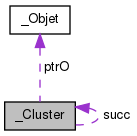
\includegraphics[scale=0.5]{images/struct_cluster.png}
\caption{Graphe de collaboration de la structure Cluster}
\end{figure} 

\subsubsection{Objet}

La structure Objet peut-\^etre représentée de la manière suivante : 
\begin{figure}[!h]
\texttt{Objet = \^\,Element;}
\paragraph{}
 \texttt{Element = enregistrement 
\begin{description}
\item idObjet : Entier non signé;
\item coordx : Entier;
\item coordy : Entire;
\item poids : Entier non signé;
\item trie : Bool
\item fin;
\end{description}
}
\caption{Représentation de la structure Objet}
\end{figure}

\paragraph{}
Un élément de la structure Objet représente un produit. Pour chaque produit, on indiquera : 
\begin{itemize}
\item[•]\textbf{l'identifiant} : idObjet
\item[•]\textbf{son coordonnée x} : coordx
\item[•]\textbf{son coordonnée y} : coordy 
\item[•]\textbf{son poids} : poids
\item[•]\textbf{s'il a déjà été trié} : trie
\end{itemize}


\subsection{Architecture}

\paragraph{}
Le programme est axé autour d'un fichier principal appelé par le main, \textit{ClusterFirst.h}. Dans le main sont aussi inclus les différentes structures citées auparavant(\ref{subsec:struct} page \pageref{subsec:struct}) ainsi que différents fichier de la librairie C. 
On peut représenter le graphe des dépendances par inclusion du main de la façon suivante : 

\begin{figure}[!h]
	\center
	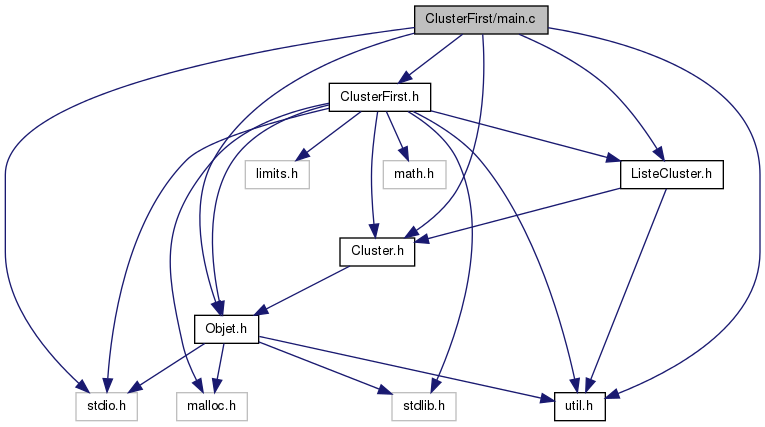
\includegraphics[scale=0.5]{images/main_inclusion.png}
	\caption{Graphe des dépendances par inclusion de \textit{main.c}}
\end{figure} 

\paragraph{}
Le main appel trois fonctions : 
\begin{itemize}
\item[•]\textbf{init} : Permet de récupérer les paramètres(capacité maximum du chariot ainsi que le fichier texte contenant les informations sur les produits, c'est à dire le carnet de commande) et affiche un message d'erreur si aucuns paramètres n'a été passé.
\item[•]\textbf{remplissageCluster} : Découpe le carnet de commande en cluster.
\item[•]\textbf{trieListeCluster} : Trie chaque cluster crée avec remplissageCluster pour que le chariot effectue l'itinéraire le plus court possible.
\end{itemize}

Le graphe d'appel du main (ci-dessous), montre tous les appels de fonction effectuer à partir celui-ci à travers les trois fonctions citées précédemment.

\begin{figure}[!h]
	\center
	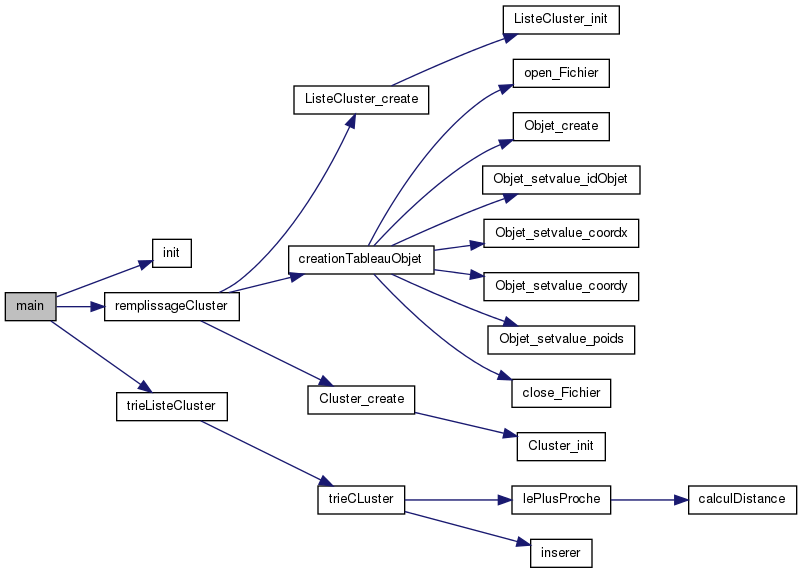
\includegraphics[scale=0.5]{images/main_appel.png}
	\caption{Graphe d'appel de la fonction main}
\end{figure}

\section{Algorithmes}

\paragraph{}
Dans cette section, les principaux différents algorithmes seront décrits.

\subsection{Remplissage des clusters}



\subsection{Trie des clusters}

%%%%%%%%%%%%%%%%%%%% CHAPITRE 3 %%%%%%%%%%%%%%%%%%%%%%

\chapter{Root First Cluster Second}

\section{Spécifications logicielles}

\section{Architecture du programme}

\section{Algorithmes}


%%%%%%%%%%%%%%%%%%%%%%% CHAPITRE 4 %%%%%%%%%%%%%%%%%%

\chapter{Test des différents heuristiques}
\label{chap:test}
%%%%%%%%%%%%%%%%%%%% CONCLUSION %%%%%%%%%%%%%%%%%%%%%%

\chapter{Conclusion}

%\annexes

\end{document}

